\chapter{Testing and Analysis}
\label{ch:testing}
\chaptermark{Fith Chapter Heading}
\newcommand{\code}[1]{\colorbox{light-gray}{\texttt{#1}}}

This chapter presents a simple feedback control system for testing, and three testing scenarios, including their execution and analysis of the results.

\section{Feedback control system description}\label{sec:test_system_description}
The system for testing is shown in Fig.~\ref{fig:tested-system}. It consists of two services:
\begin{enumerate}
    \item Order management service. It is simple web service that has two HTTP~\cite{http} methods: one for creating order directly (GET api/order) and another for creating order for delivery (GET api/order-delivery). Both methods has been artificially delayed, such that the response time averages 250 milliseconds. Also this service is artificially restricted and it can hold only 10 requests simultaneously.
    \item Delivery management service. It has one HTTP~\cite{http} method GET api/delivery. This method synchronously calls the GET api/order-delivery method of order management service method and with success. Responce timeout is equal to 5 seconds.
\end{enumerate}

The method for creating orders directly is a critical component of the tested system.
Therefore, in the event of increased traffic, it should be made available as a priority. Due to the fact that the delivery management service also uses this service via another method, it may be necessary to restrict its in the event of risks of unavailability.

Therefore, delivery management service use circuit breaker pattern from the resilience4j~\cite{resilience4j} library for calling the GET api/order method. It starts with the closed state and counts the number of errors in the specified interval (sliding window). If the percentage of error exceeds a predetermined threshold, it will open and block all incoming requests. After a certain period of time, it will partially open and allow a limited number of requests to test. If these requests meet the error threshold criteria, the circuit breaker will close. Otherwise, it will return to the open state. This implementation of circuit breaker has the following main configuration parameters:
\begin{enumerate}
    \item \textbf{slidingWindowSize}. The duration of time for which errors are counted.
    \item \textbf{failureRateThreshold}. Percentage of errors for transition to a open state.
    \item \textbf{waitDurationInOpenState}. The waiting duration before transition from open to half-open state
    \item \textbf{permittedNumberOfCallsInHalfOpenState}. The number of permitted calls to the half-open state to test whether the circuit breaker can be closed.
\end{enumerate}

\begin{figure}[t]
    \centering
    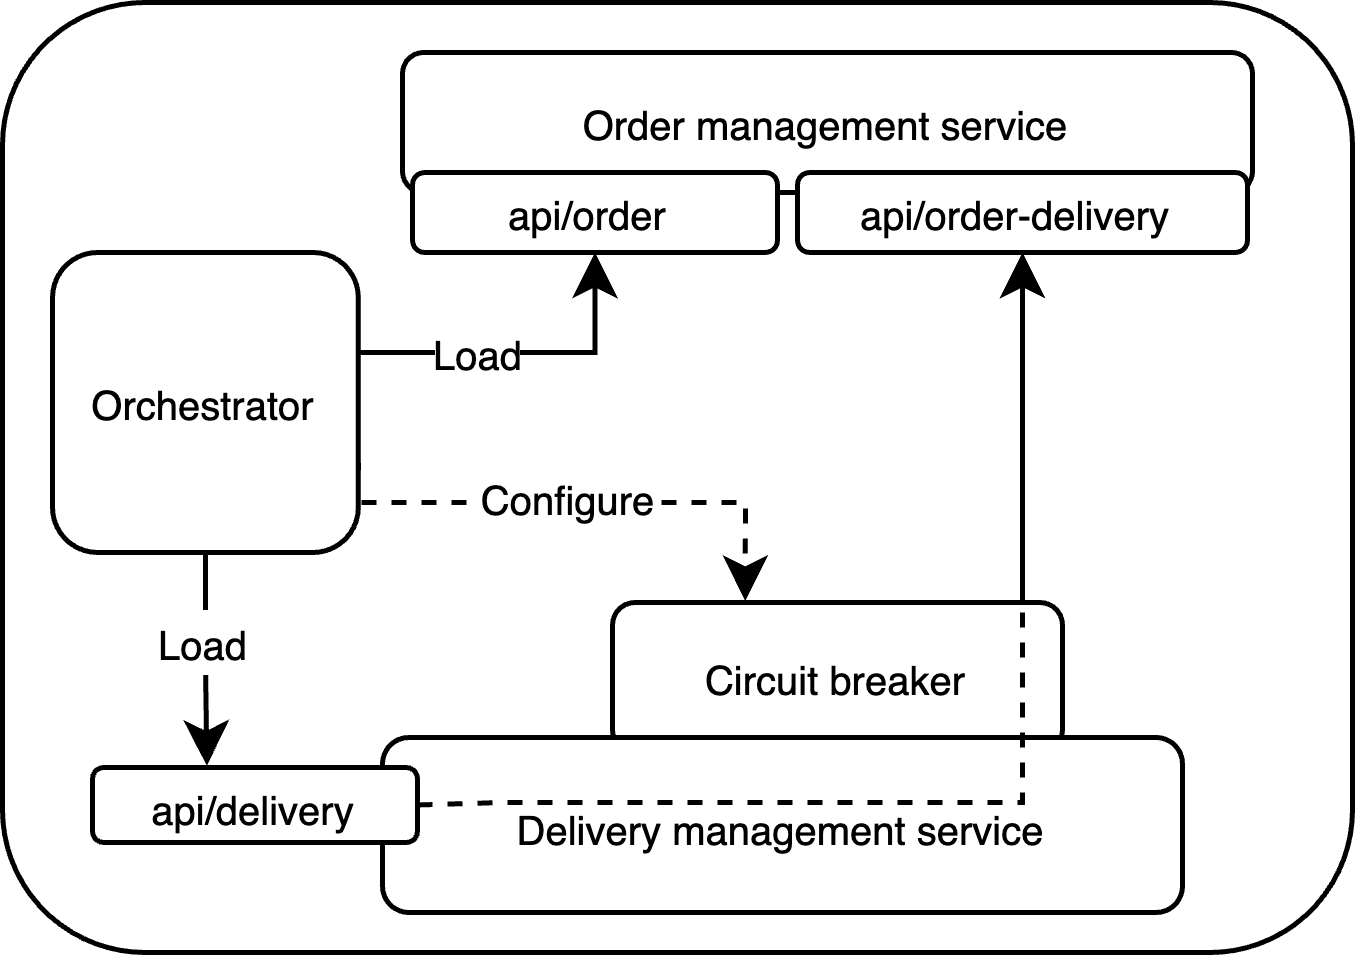
\includegraphics[height=\textheight,width=\textwidth,keepaspectratio]{tested_system.png}
    \caption{Tested system}
    \label{fig:tested-system}
\end{figure}


For testing purposes, I set the slidingWindowSize to 5 seconds, the waitDurationInOpenState to 60 seconds, and the permittedNumberOfCallsInHalfOpenState set to 10. The aim of the testing was to access the behavior of the circuit breaker under the different values of the failureRateThreshold parameter. Additionally, to test the circuit breaker under the similar condition the load generation configuration was the same for all test scenarios. This configuration is presented on the Listing~\ref{lst:load_config}
\lstinputlisting[caption=Load configuration, label={lst:load_config}]{code/load.yaml}
The order management service experiences a constant load of 10 RPS for 4 minutes, accessing the GET api/order endpoint.
The delivery management service initially has a load of 20 RPS, which then increases sharply to 200 RPS within 2 minutes, before returning to a constant 10 RPS level for 1 minute.

\section{The first scenario}\label{sec:test_description_1}
For the first scenario the error threshold was equal to 90\%.
The full configuration of the circuit breaker for the first test is presented on Listing~\ref{lst:cb_1}
\lstinputlisting[caption=Configuration of the circuit breaker for the first test, label={lst:cb_1}]{code/cb1.yaml}


With such a high threshold, the circuit breaker is expected to open at the end of test, when fewer than 10\% of the requests are successful.
However, the results differ from the assumptions.
Fig~\ref{fig:response-cb-90} shows the response time of the services in relation to time and the number of the requests per second. The green line represents the response time of the delivery management service, and the yellow line represents the order management service.
Fig.~\ref{fig:http-cb-90} indicates that, as the load increases, the number of errors also increases.
Fig.~\ref{fig:error-cb-90} illustrates the error percentage for the last 5 seconds. The highest value is approximately 80\%.
Therefore, the circuit breaker in this scenario did not even open to protect the order management service from overload.

\begin{figure}[t]
    \centering
    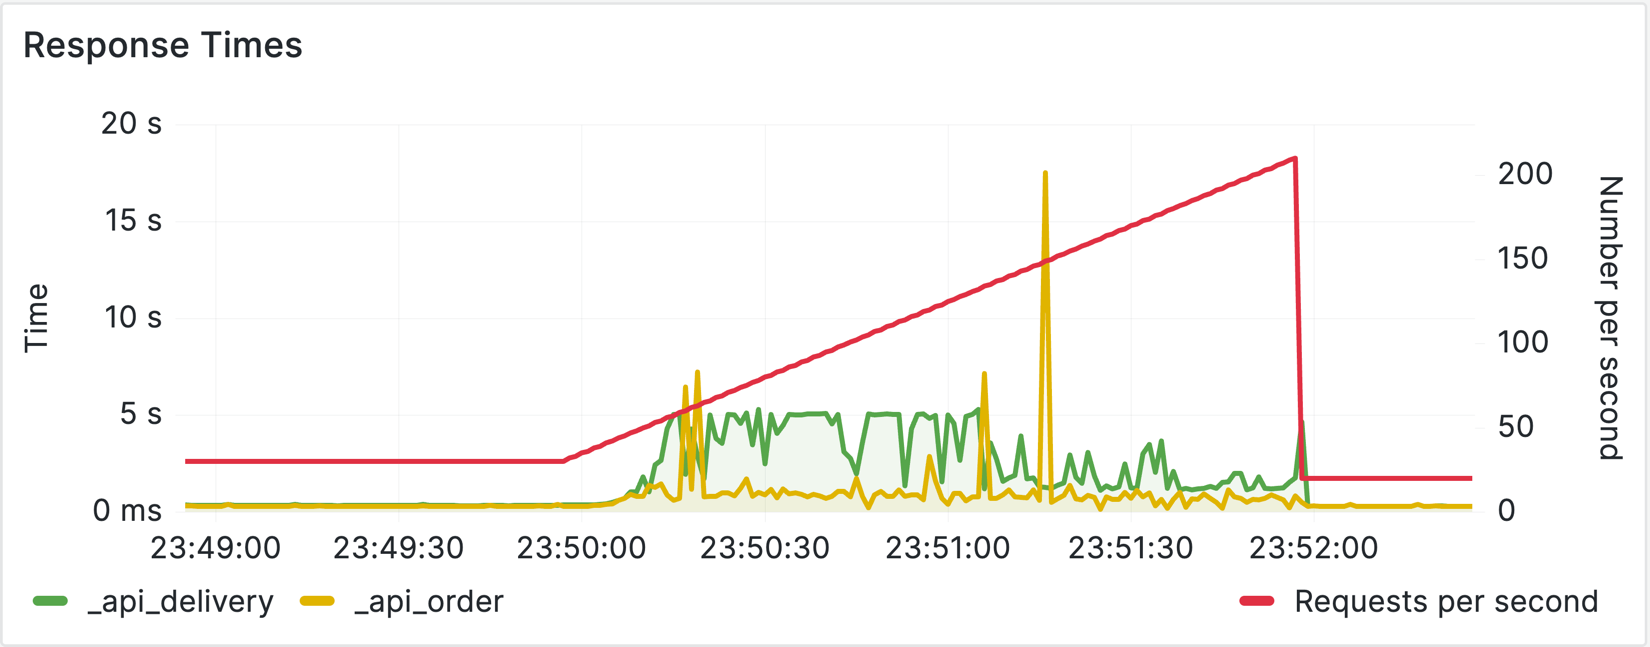
\includegraphics[height=\textheight,width=\textwidth,keepaspectratio]{response_cb_90.png}
    \caption{Response time of the services when error threshold is equal to 90\%}
    \label{fig:response-cb-90}
\end{figure}
\begin{figure}[t]
    \centering
    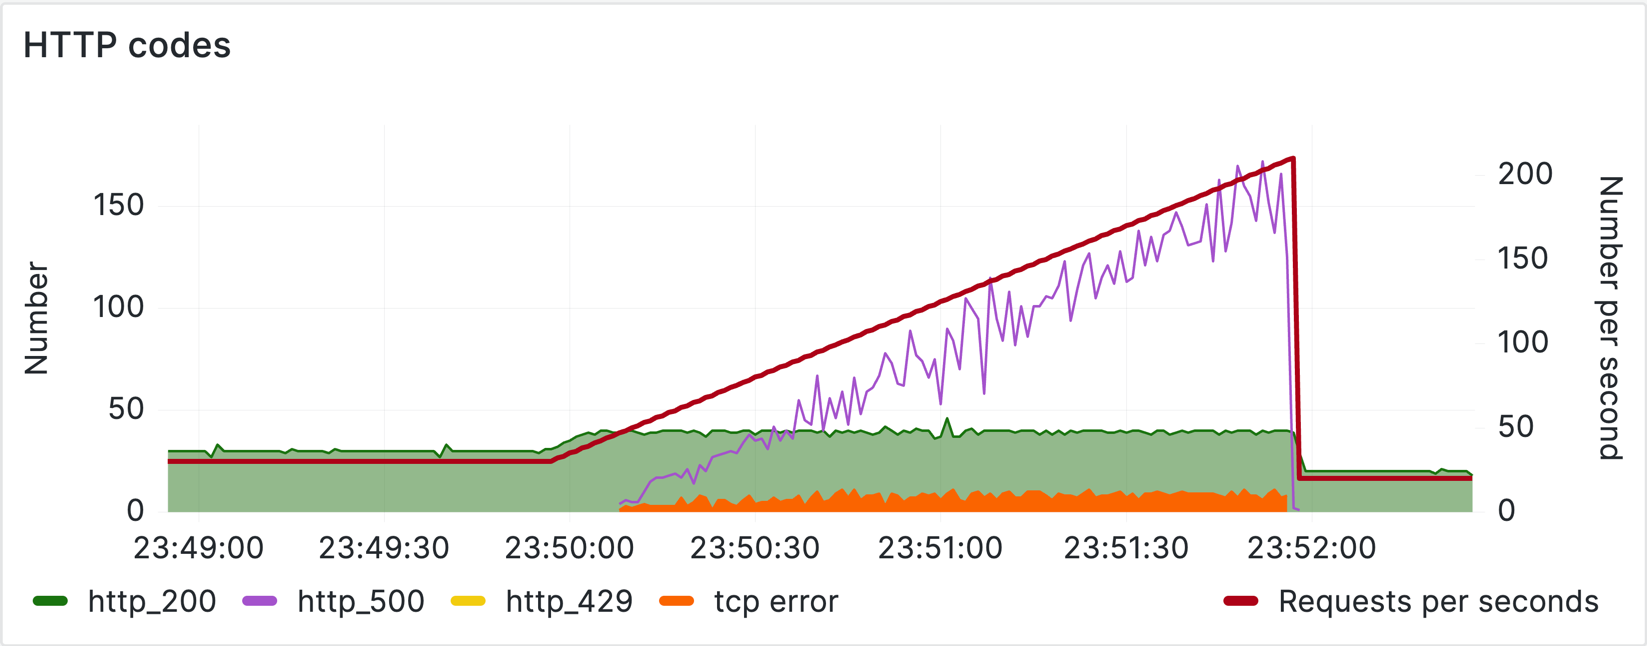
\includegraphics[height=\textheight,width=\textwidth,keepaspectratio]{http_cb_90.png}
    \caption{HTTP codes responces when error threshold is equal to 90\%}
    \label{fig:http-cb-90}
\end{figure}
\begin{figure}[t]
    \centering
    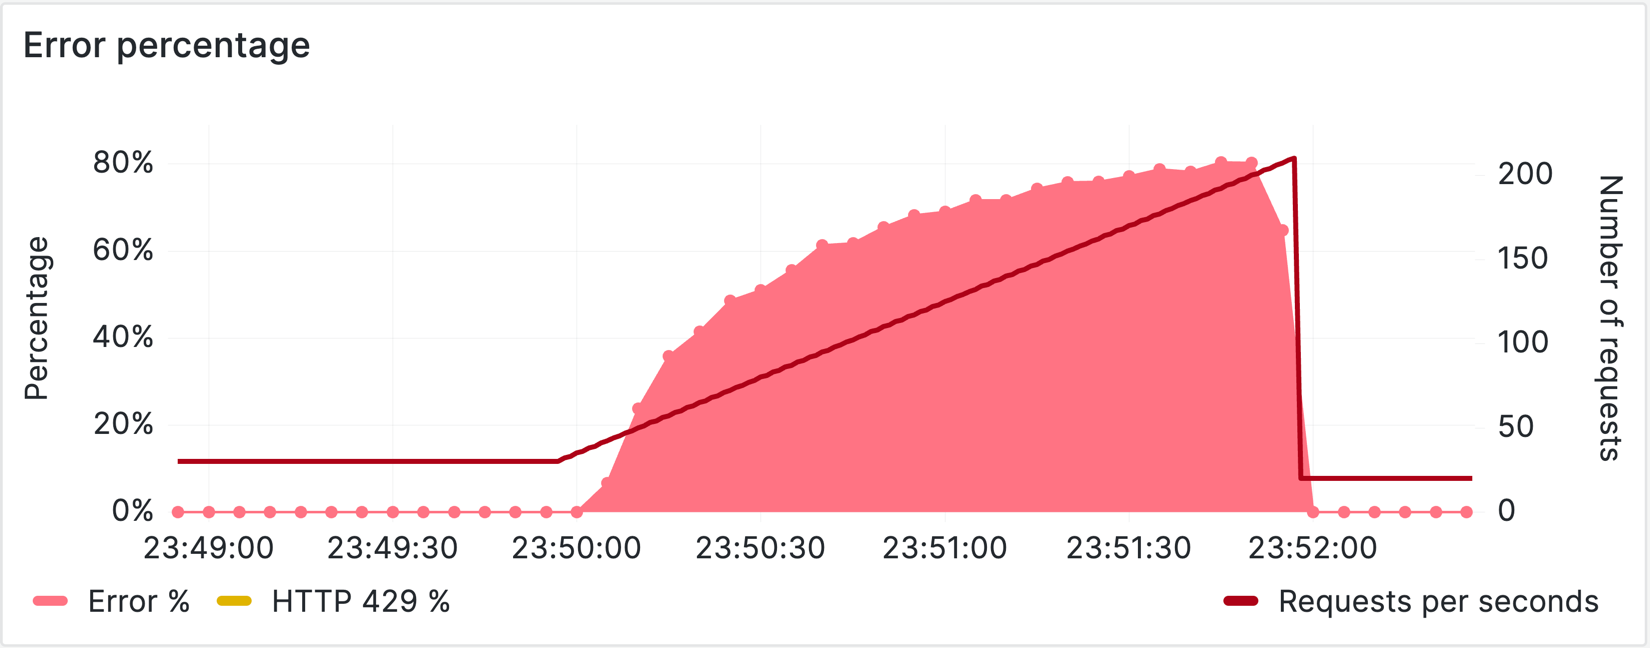
\includegraphics[height=\textheight,width=\textwidth,keepaspectratio]{error_cb_90.png}
    \caption{Percentage error response when error threshold is equal to 90\%}
    \label{fig:error-cb-90}
\end{figure}

\section{The second scenario}\label{sec:test_description_2}
For the second scenario the error threshold was equal to 15\%.
The full configuration of the circuit breaker for the second test is presented on Listing~\ref{lst:cb_2}
\begin{minipage}{\textwidth}
\lstinputlisting[caption=Configuration of the circuit breaker for the second test, label={lst:cb_2}]{code/cb2.yaml}
\end{minipage}

The Fig~\ref{fig:response-cb-15} shows that immediately after increasing the load, the circuit breaker opens.
Fig~\ref{fig:error-cb-15} and Fig~\ref{fig:http-cb-15} show that after 15\% threshold is exceeded, services stop responding with errors.

\begin{figure}[t]
    \centering
    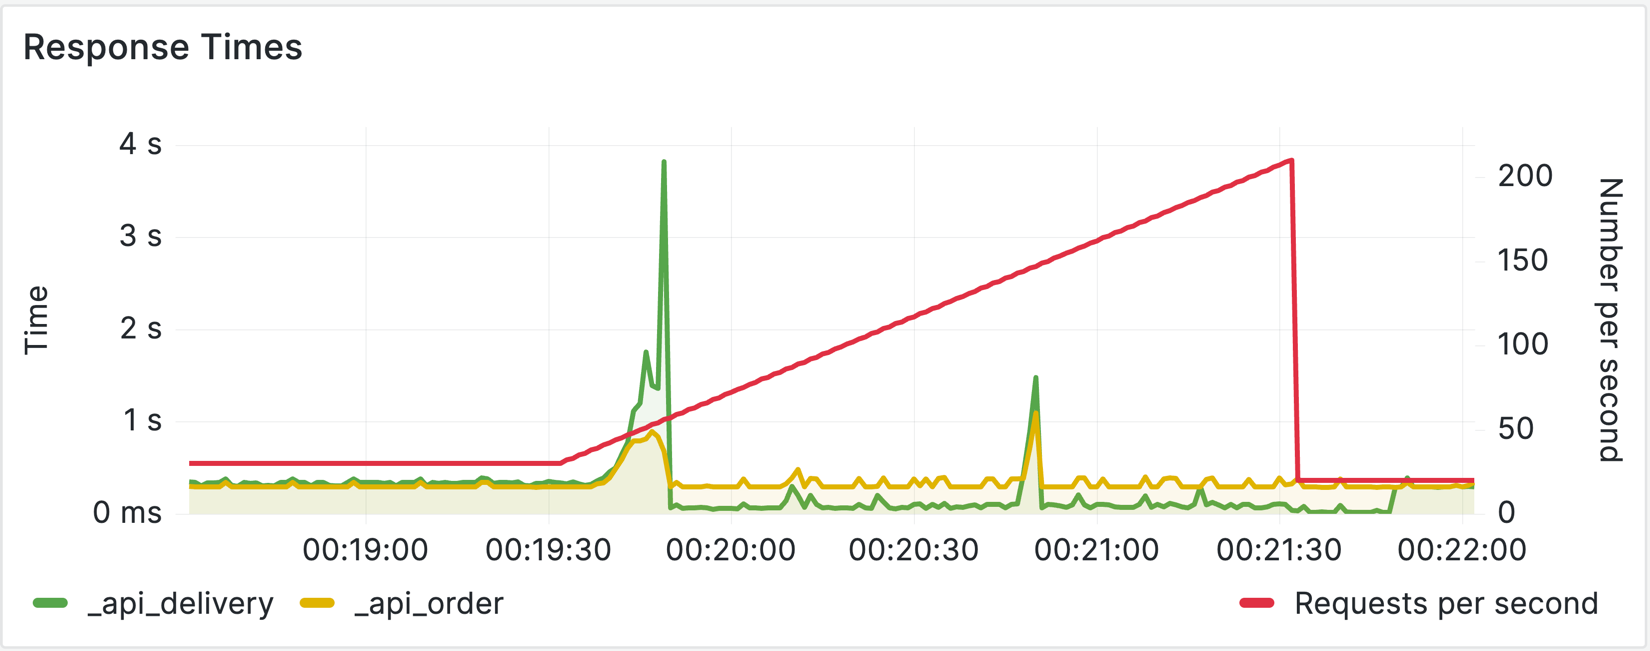
\includegraphics[height=\textheight,width=\textwidth,keepaspectratio]{response_cb_15.png}
    \caption{Response time of the services when error threshold is equal to 15\%}
    \label{fig:response-cb-15}
\end{figure}
\begin{figure}[t]
    \centering
    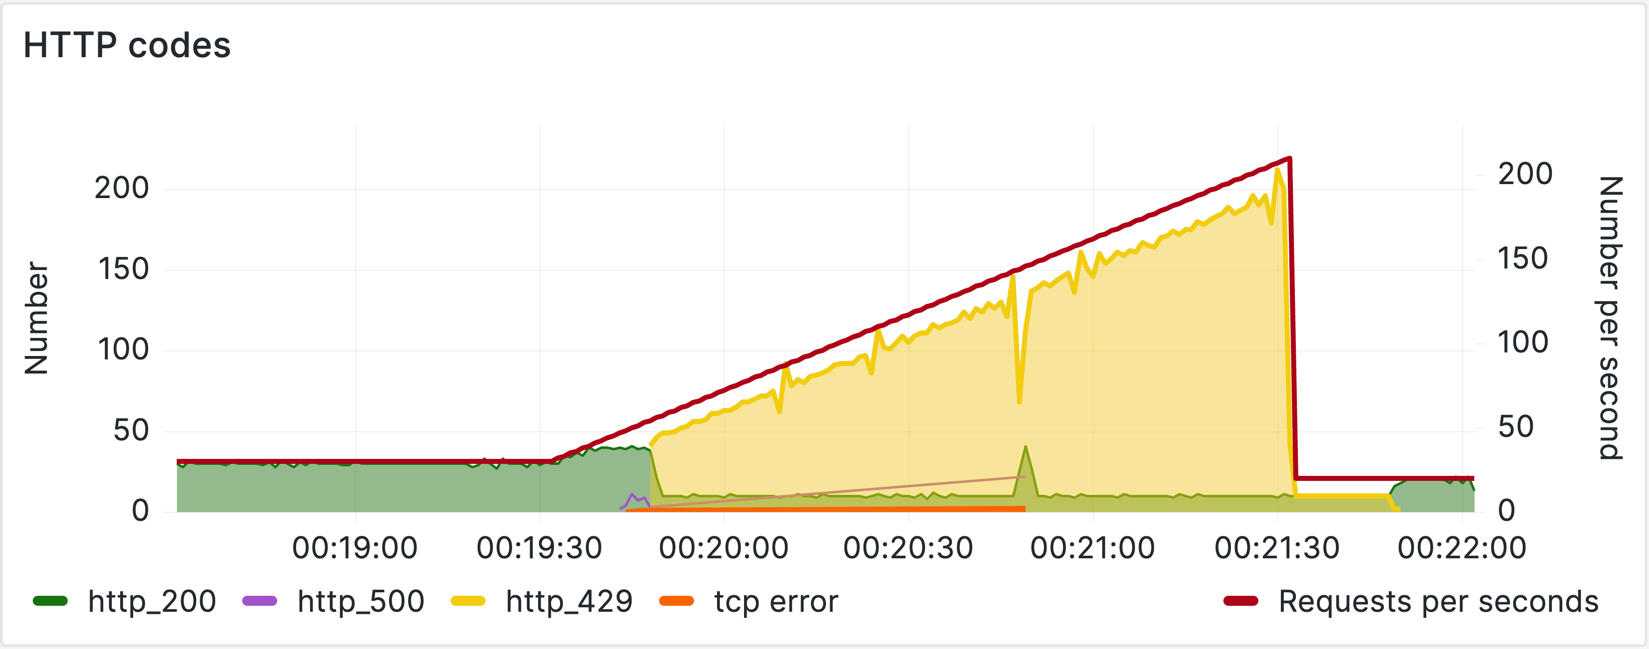
\includegraphics[height=\textheight,width=\textwidth,keepaspectratio]{http_cb_15.png}
    \caption{HTTP codes responces when error threshold is equal to 15\%}
    \label{fig:http-cb-15}
\end{figure}
\begin{figure}[t]
    \centering
    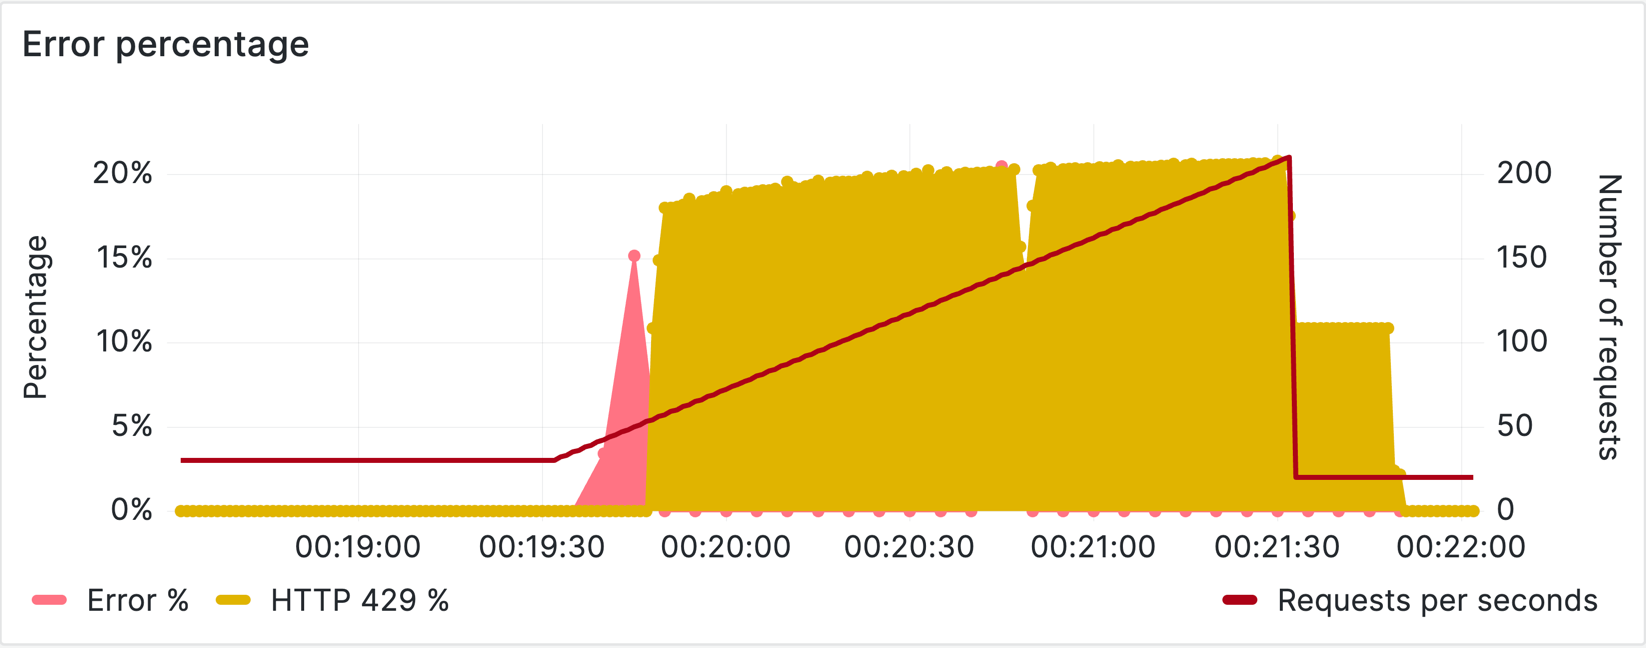
\includegraphics[height=\textheight,width=\textwidth,keepaspectratio]{error_cb_15.png}
    \caption{Percentage error response when error threshold is equal to 15\%}
    \label{fig:error-cb-15}
\end{figure}

\section{The third scenario}\label{sec:test_description_3}
The configuration of the circuit breaker for the third scenario is presented on Listing~\ref{lst:cb_3}
\begin{minipage}{\textwidth}
\lstinputlisting[caption=Configuration of the circuit breaker for the third test, label={lst:cb_3}]{code/cb3.yaml}
\end{minipage}

The Fig~\ref{fig:response-cb-50} shows that after the start of the load increasing, the approximately 30 seconds is passed.
Fig~\ref{fig:error-cb-50} and Fig~\ref{fig:http-cb-50} show that after 50\% threshold is exceeded, services stop responding with errors. These results indicates that circuit breaker with the third configuration was really waiting until the error threshold reached 50\%.
\begin{figure}[t]
    \centering
    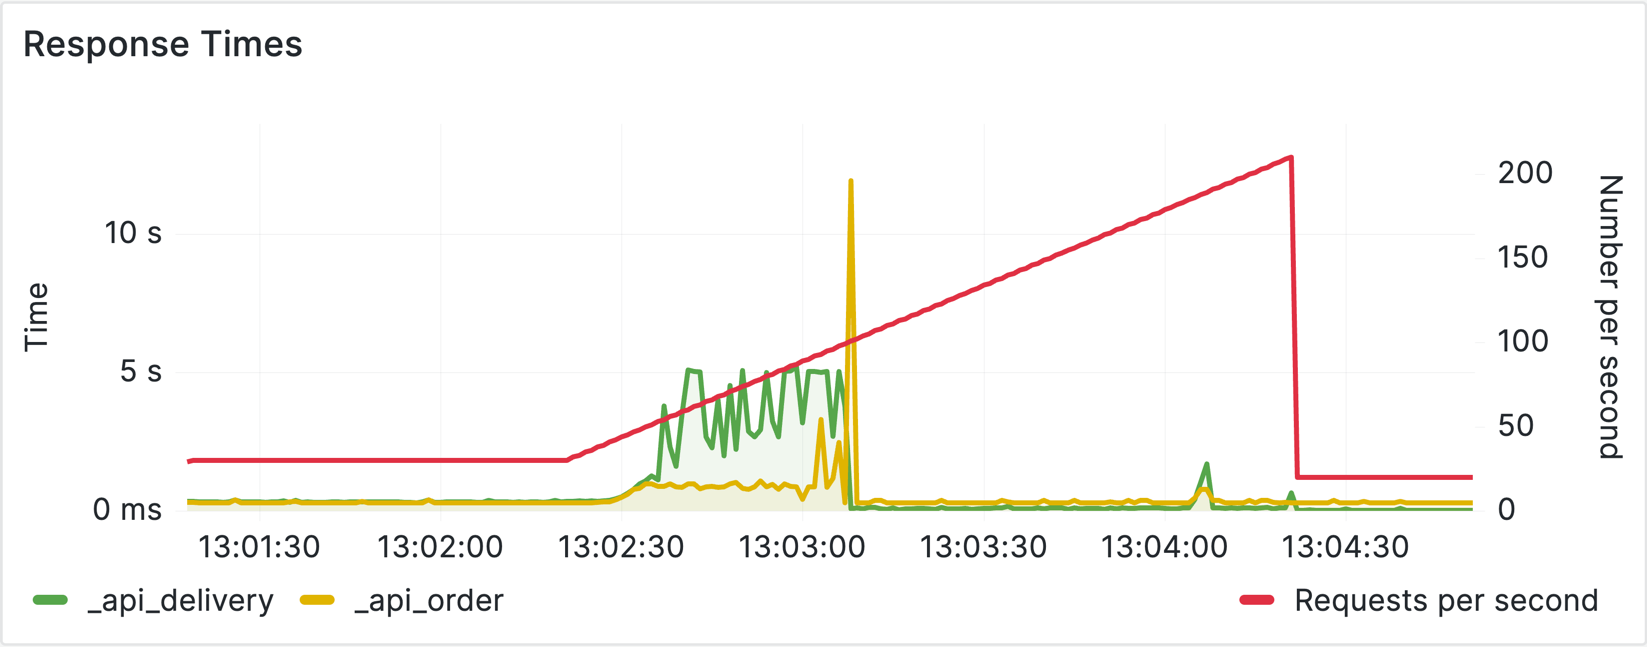
\includegraphics[height=\textheight,width=\textwidth,keepaspectratio]{response_cb_50.png}
    \caption{Response time of the services when error threshold is equal to 50\%}
    \label{fig:response-cb-50}
\end{figure}

\begin{figure}[t]
    \centering
    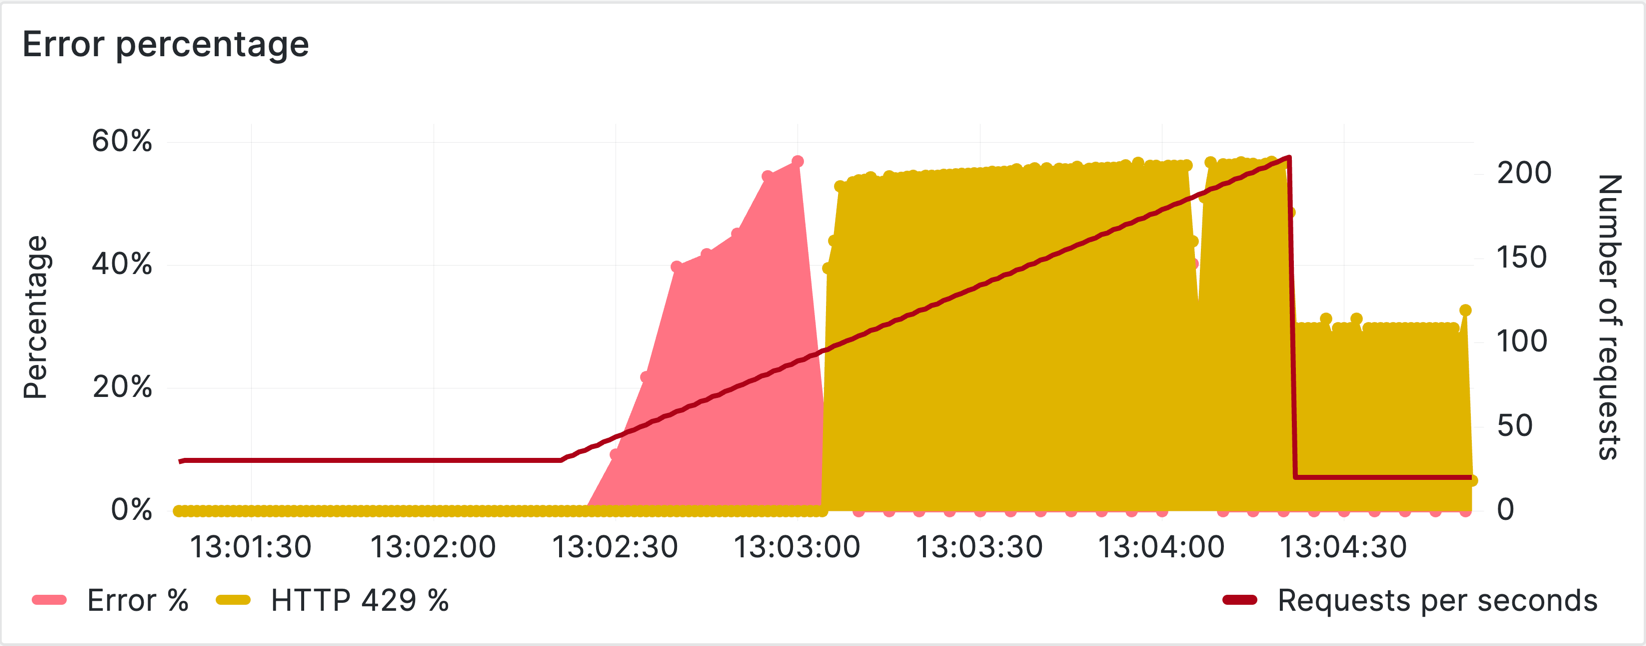
\includegraphics[height=\textheight,width=\textwidth,keepaspectratio]{error_cb_50.png}
    \caption{HTTP codes responces when error threshold is equal to 50\%}
    \label{fig:error-cb-50}
\end{figure}

\begin{figure}[t]
    \centering
    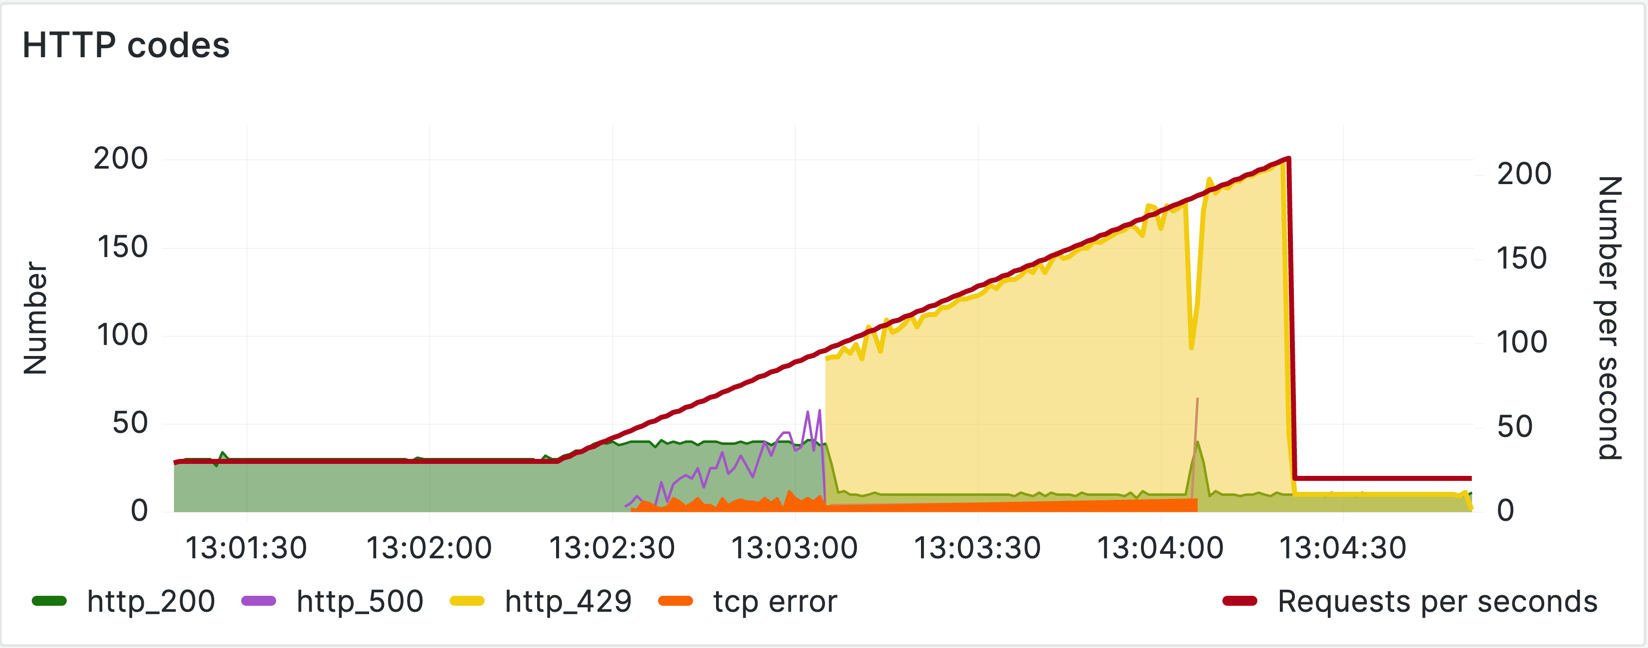
\includegraphics[height=\textheight,width=\textwidth,keepaspectratio]{http_cb_50.png}
    \caption{Percentage error response when error threshold is equal to 50\%}
    \label{fig:http-cb-50}
\end{figure}

\section{Analysis}\label{sec:analysis}
Three scenarios were used to test the implementation of a circuit breaker from the resilience4j library, or
rather, how accurately the circuit breaker taked into account the error threshold parameter. The first test showed that the system
under the described scenario did not exceed 80\% of errors, and the circuit breaker with a 90\% error threshold did not
open. Subsequent tests with thresholds 15\% and 50\% for circuit breaker demonstrated that it opened
at the correct point and prevented order management system from overload.

